\subsection[Regressione Logistica]{\textit{Regressione Logistica}}

%\subsubsection[Training e test set]{Training e test set}


\begin{frame}
	
	\frametitle{Regressione Logistica}
	
%	Ma un modello di machine learning mira a fare \textbf{buone previsioni su dati nuovi} e mai visti prima.
%	Ma se stai costruendo un modello dal tuo dataset, come potresti ottenere dei dati precedentemente non visti?\vspace{3mm}
%	\pause
%	
%	Un modo è \textbf{dividere il dataset in due sottoinsiemi}:
%	\begin{itemize}
%		\item \textbf{training-set}, un sottoinsieme per addestrare un modello
%		\item \textbf{test-set}, un sottoinsieme per testare il modello addestrato
%	\end{itemize}
%	\ \\
%	Una buona prestazione sul test set è un utile indicatore di buone prestazioni su dei nuovi dati in generale, supponendo che:
%	\begin{itemize}
%		\item il test-set sia abbastanza grande per produrre risultati statisticamente significativi
%		\item non imbrogli usando lo stesso test-set più e più volte
%		\item è rappresentativo dell'insieme di dati nel suo complesso
%	\end{itemize}

	
	\begin{columns}
		\column{0.8\linewidth}
		Immaginiamo per un secondo di avere il problema di prevedere la probabilità di testa per alcuni lanci di moneta dove forse la moneta è leggermente piegata.
	
		Potresti usare features come:
		\begin{itemize}
			\item angolo di piegatura
			\item massa della moneta
			\item o simili
		\end{itemize}
			
		\column{0.2\linewidth}
		\begin{figure}[!htbp]
			\centering
			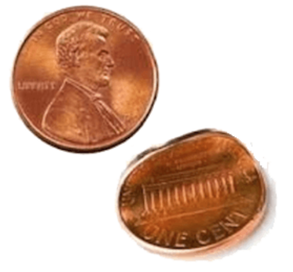
\includegraphics[width=1.0\linewidth]{images/supervised/z_algoritms_logistic_regression/flipped_coin.png}
%			\caption{}
		\end{figure}			
	\end{columns}
	\ \\
	Qual è il modello più semplice che potresti pensare di utilizzare?
	\newlinedouble
	Potremmo usare la regressione lineare.\\
	Ma utilizzando tale modello potremmo avere degli strani risultati...\\
	Ad esempio, cosa succede se abbiamo una nuova moneta che ha una massa molto pesante, che non abbiamo mai visto prima?\\
	E cosa succede se abbiamo un angolo estremamente grande?
\end{frame}


\begin{frame}
	
	\frametitle{Regressione Logistica}
	
	Potremmo ottenere previsioni che sono al di \textbf{fuori dell'intervallo tra 0 e 1}.
	\newlinedouble
	Le probabilità sono limitate tra 0 e 1 e se abbiamo un modello di previsione che ci dà un valore al di fuori di tale intervallo, saremo nei guai...\\
	Soprattutto se stabiliamo di provare a moltiplicare le probabilità predette o di usarle per creare valori attesi, cose del genere.
	\newlinedouble
	Bene, come primo hack, potresti provare a bloccare quella previsione per ignorare eventuali valori anomali (minori di 0 o maggiori di 1).
	\newlinedouble
	Quindi la cosa giusta da fare è inventare una funzione di perdita e un metodo di previsione leggermente diversi.
	Ciò consente ai nostri valori di essere interpretati naturalmente come probabilità da 0 a 1 e non supera mai tale intervallo tra 0 a 1.
	Quindi chiamiamo questa idea \textbf{regressione logistica}.
\end{frame}


\begin{frame}
	
	\frametitle{Regressione Lineare vs Regressione Logistica}
	\begin{figure}[!htbp]
		\centering
		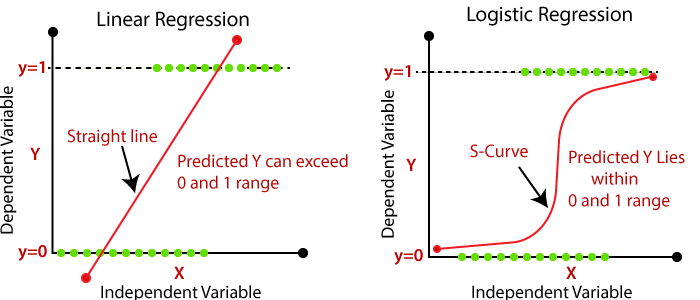
\includegraphics[width=1.0\linewidth]{images/supervised/z_algoritms_logistic_regression/linear-regression-vs-logistic-regression.png}
		%\caption{Stima della probabilità di fallimento di un cliente sulla base del saldo}
	\end{figure}
	
\end{frame}


\begin{frame}
	
	\frametitle{Regressione Lineare vs Regressione Logistica: un caso reale}
	\begin{figure}[!htbp]
		\centering
		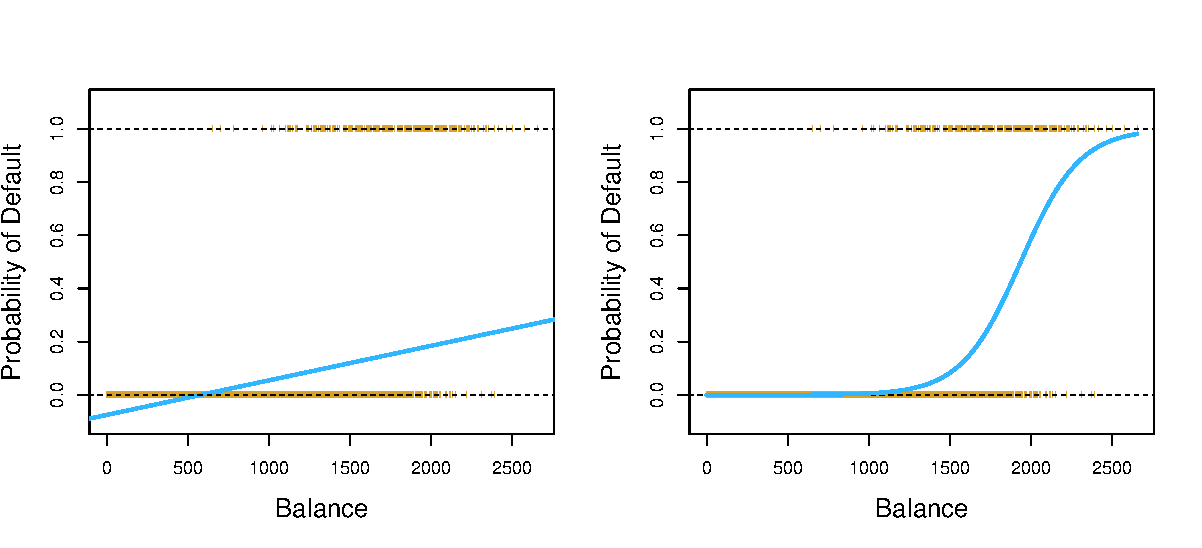
\includegraphics[width=1.0\linewidth]{images/supervised/z_algoritms_logistic_regression/linear_vs_logistic}
		\caption{Stima della probabilità di fallimento di un cliente sulla base del saldo}
	\end{figure}
	
\end{frame}


\begin{frame}
	
	\frametitle{Regressione Logistica}
	
	La regressione logistica è un meccanismo estremamente efficiente per il calcolo delle probabilità.
	\newlinedouble
	In pratica, puoi utilizzare la probabilità restituita in uno dei due modi:
	\begin{itemize}
		\item ``così come è'' (utile ad esempio per calcolare valori attesi)
		\item convertito in una categoria binaria (definendo una soglia di split)
	\end{itemize}
	\ \\
	Ci si potrebbe chiedere come un modello di regressione logistica possa garantire un output che è sempre compreso tra 0 e 1.\\
	In effetti, una funzione sigmoide, definita come segue, produce un output con le suddette caratteristiche.

	%Prendiamo il nostro modello lineare classico e lo inseriamo in un sigmoide.

\end{frame}


\subsubsection[Il sigmoide]{Il sigmoide}
\begin{frame}
	
	\frametitle{Regressione Logistica: il sigmoide}
	
	\begin{empheq}[box=\fcolorbox{blue!40!black!60}{yellow!10}]{align*}
	\pmb{\text{Il sigmoide}} \quad \Rightarrow \quad y' = \frac{1}{1 + e^{-z}} = \frac{e^z}{1 + e^z} \quad \text{ dove } \quad z = \omega^Tx+b
	\end{empheq}
	
	\begin{columns}
		\column{0.55\linewidth}	
		Si noti che $z$ è spesso indicato come il \textbf{log-odds} perché  l'inverso del sigmoide afferma che z può essere definito come:
		\begin{itemize}
			\item il logaritmo della probabilità della label ``1'' (es: ``testa'')
			\item diviso per la probabilità della label ``0'' (es: ``croce'')
			\item ricordando che $log_a (b^c) = c\text{ }log_a (b)$
		\end{itemize}
		\ \\
		Ovvero:
		\column{0.45\linewidth}
		\begin{figure}[!htbp]
			\centering
			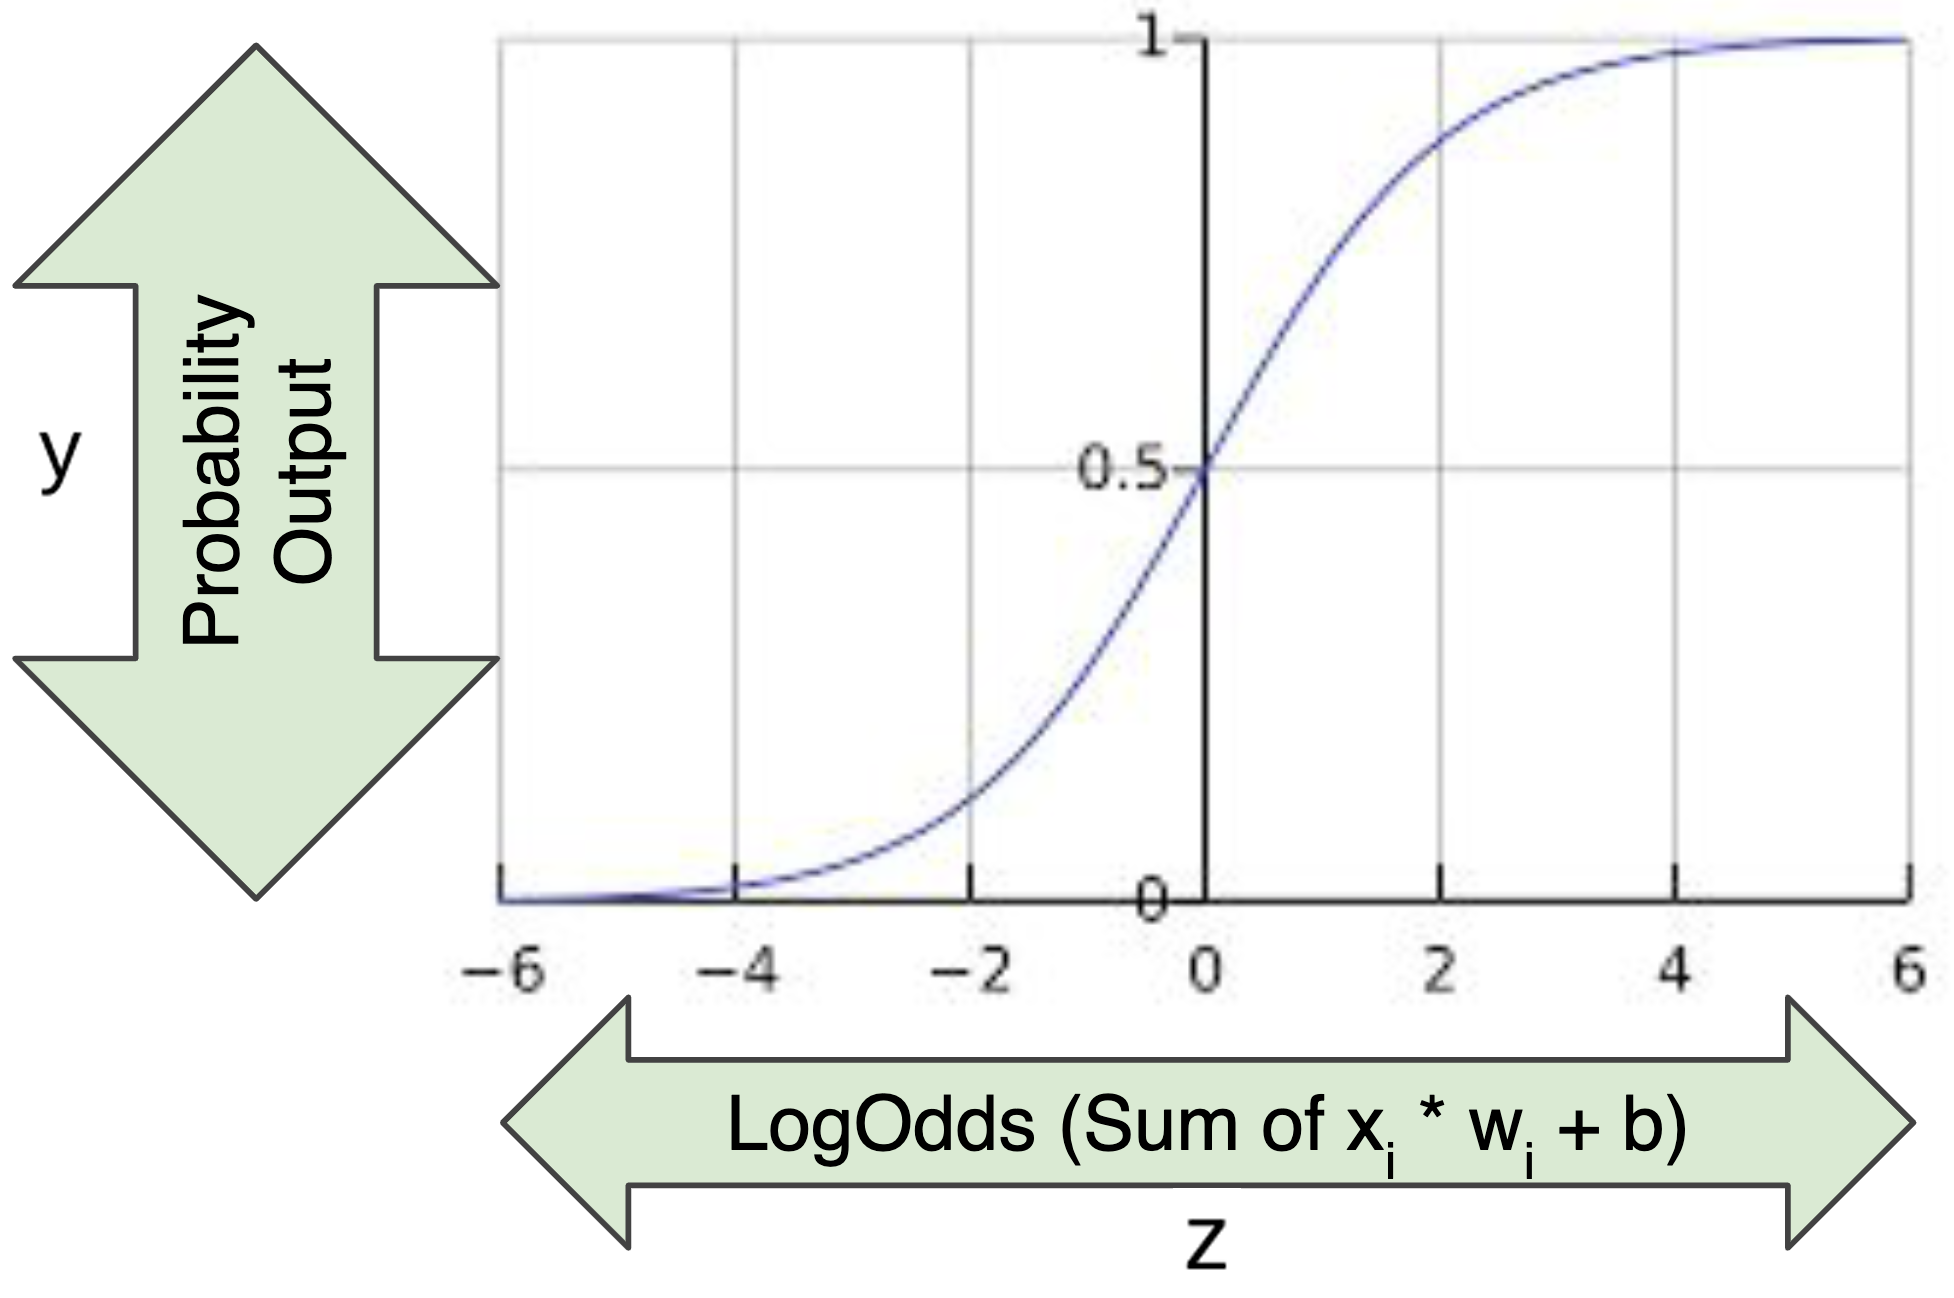
\includegraphics[width=1.0\linewidth]{images/supervised/z_algoritms_logistic_regression/SigmoidFunction.png}
	%		\caption{Sigmoid Function}
		\end{figure}
		
%		\begin{figure}[!htbp]
%			\centering
%			\includegraphics[width=1.0\linewidth]{images/supervised/z_algoritms_logistic_regression/log_proprieta_3.png}
%	%		\caption{Sigmoid Function}
%		\end{figure}
	\end{columns}
	
	\begin{empheq}[box=\fcolorbox{blue!40!black!60}{yellow!10}]{align*}
	\pmb{\text{Il log-odds (o logit)}} \quad \Rightarrow \quad z = log \left(\frac{y'}{1-y'} \right) = \omega^Tx + b
	\end{empheq}
	
\end{frame}


\begin{frame}
	
	\frametitle{Regressione Logistica: un esempio parte 1}
	
	Supponiamo di avere un modello di regressione logistica con tre caratteristiche che apprendano i seguenti bias e pesi:
	\begin{itemize}
		\item $b = 1$
		\item $\omega_1 = 2$
		\item $\omega_2 = -1$
		\item $\omega_3 = 5$
	\end{itemize}
	
	Supponiamo inoltre i seguenti valori delle features per un dato esempio:
	\begin{itemize}
		\item $x_1 = 0$
		\item $x_2 = 10$
		\item $x_3 = 2$
	\end{itemize}
	
\end{frame}


\begin{frame}
	
	\frametitle{Regressione Logistica: un esempio parte 2}

	\begin{columns}
		\column{0.55\linewidth}	
		Pertanto, il log-odds:
		$$b + \omega_1x_1 + \omega_2x_2 + \omega_3x_3$$
	
		sarà:
		$$(1) + (2)(0) + (-1)(10) + (5)(2) = 1$$	
		
		Di conseguenza, la previsione della regressione logistica per questo particolare esempio sarà $0.731$:
		$$y' = \frac{1}{1 + e^{-(1)}} = 0.731$$
		
		\column{0.45\linewidth}
		\begin{figure}[!htbp]
			\centering
			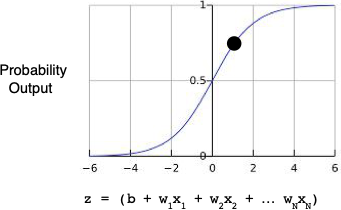
\includegraphics[width=1.0\linewidth]{images/supervised/z_algoritms_logistic_regression/LogisticRegressionOutput0_731.png}
			\caption{Probabilità dello 0.731}
		\end{figure}
	\end{columns}
	
\end{frame}


\subsubsection[Log Loss]{Log Loss}

\begin{frame}
	
	\frametitle{Regressione Logistica: Log Loss}

	La loss per la regressione lineare è la loss quadratica.\\
	La loss per la regressione logistica è \textbf{Log Loss}, definita come segue:
	\begin{empheq}[box=\fcolorbox{blue!40!black!60}{yellow!10}]{align*}
	\pmb{\text{Log Loss}} = \sum_{(x,y)\in D} -y\log(y') - (1 - y)\log(1 - y')
	\end{empheq}
	
	Dove:
	\begin{itemize}
		\item $(x,y)\in D$ è il dataset contenente molte coppie di esempi etichettati
		\item $y$ è l'etichetta di un esempio etichettato. Poiché si tratta di regressione logistica, ogni valore di y deve essere $0$ o $1$.
		\item $y'$ è il valore previsto (da qualche parte tra 0 e 1), dato l'insieme delle features $x$
	\end{itemize}
	
\end{frame}


\begin{frame}
	
	\frametitle{Regressione Logistica: un esempio grafico 1 con GD}
	
	%\begin{block}{}
		\centering
		\animategraphics[controls={play, step, stop}, height=7cm]{6.0}{images/supervised/z_algoritms_logistic_regression/logistic_regression_gd/logistic_regression_gd-}{0}{124}
	%\end{block}

\end{frame}


\begin{frame}
	
	\frametitle{Regressione Logistica: un esempio grafico 2 con GD}
	
	%\begin{block}{}
		\centering
		\animategraphics[controls={play, step, stop}, height=7cm]{6.0}{images/supervised/z_algoritms_logistic_regression/logistic_regression_gd_2/logistic_regression_gd_2-}{0}{133}
	%\end{block}

\end{frame}


\subsubsection[Regolarizzazioni $L_2$ e $\lambda$]{Regolarizzazione $L_2$ e $\lambda$}

\begin{frame}
	
	\frametitle{Regressione Logistica: regolarizzazioni}

	La maggior parte dei modelli di regressione logistica utilizza una delle seguenti due strategie per smorzare la complessità del modello:
	\begin{itemize}
		\item una regolarizzazione $L_2$
		\item un arresto anticipato, limitando il numero degli step di addestramento o il tasso di apprendimento
	\end{itemize}
	\ \\
	L'idea alla base delle regolarizzazioni è la seguente;
	invece di mirare semplicemente a ridurre al minimo la loss (minimizzazione empirica del rischio):
	\begin{empheq}[box=\fcolorbox{blue!40!black!60}{yellow!10}]{align*}
	\text{minimize(Loss(Data|Model))}
	\end{empheq}
	cerchiamo di minimizzare la loss+complessità che prende il nome di \textbf{structural risk minimization}:
	\begin{empheq}[box=\fcolorbox{blue!40!black!60}{yellow!10}]{align*}
	\text{minimize(Loss(Data|Model) + complexity(Model))}
	\end{empheq}
\end{frame}


\begin{frame}
	
	\frametitle{Regressione Logistica: regolarizzazioni}

	Il nostro algoritmo di ottimizzazione è ora una funzione di due termini: il \textbf{termine di loss}, che misura quanto bene il modello si adatta ai dati, e il \textbf{termine di regolarizzazione}, che misura la complessità del modello.
	\newlinedouble
	Due tecniche di regolarizzazione piuttosto comuni per valutare la complessità del modello sono:
	\begin{itemize}
		\item la complessità del modello come funzione dei pesi di tutte le funzionalità del modello
		\item complessità del modello in funzione del numero totale di elementi con pesi diversi da zero
	\end{itemize}
	
	\ \\
	La regolarizzazione è estremamente importante nella modellazione della regressione logistica. Senza regolarizzazione, la natura asintotica della regressione logistica continuerebbe a portare la loss verso lo 0 nelle dimensioni elevate.

\end{frame}


\begin{frame}
	
	\frametitle{Regressione Logistica: regolarizzazione $L_2$ e $\lambda$}

	Possiamo quantificare la complessità utilizzando la formula di regolarizzazione $L_2$, che definisce il termine di regolarizzazione come la somma dei quadrati di tutti i pesi delle caratteristiche:
	\begin{empheq}[box=\fcolorbox{blue!40!black!60}{yellow!10}]{align*}
	L_2\text{ regularization term} = ||\boldsymbol w||_2^2 = {w_1^2 + w_2^2 + ... + w_n^2}
	\end{empheq}
	
	In questa formula, i pesi vicini allo zero hanno scarso effetto sulla complessità del modello, mentre i pesi anomali possono avere un impatto enorme.
	\newlinedouble
	Gli sviluppatori di modelli ottimizzano l'impatto complessivo del termine di regolarizzazione moltiplicando il suo valore per uno scalare noto come lambda (chiamato anche tasso di regolarizzazione).\\
	Ovvero, gli sviluppatori di modelli mirano a fare quanto segue:
	\begin{empheq}[box=\fcolorbox{blue!40!black!60}{yellow!10}]{align*}
	\text{minimize(Loss(Data|Model)} + \lambda \text{ complexity(Model))}
	\end{empheq}
\end{frame}